\documentclass[a4paper,11pt,oneside]{memoir}

% Castellano
\usepackage[spanish,es-tabla]{babel}
\selectlanguage{spanish}
\usepackage[utf8]{inputenc}
\usepackage{placeins}

\RequirePackage{booktabs}
\RequirePackage[table]{xcolor}
\RequirePackage{xtab}
\RequirePackage{multirow}

% Links
\usepackage[colorlinks]{hyperref}
\hypersetup{
	allcolors = {red}
}

% Ecuaciones
\usepackage{amsmath}

% Rutas de fichero / paquete
\newcommand{\ruta}[1]{{\sffamily #1}}

% Párrafos
\nonzeroparskip


% Imagenes
\usepackage{graphicx}
\newcommand{\imagen}[2]{
	\begin{figure}[!h]
		\centering
		\includegraphics[width=0.9\textwidth]{#1}
		\caption{#2}\label{fig:#1}
	\end{figure}
	\FloatBarrier
}

\newcommand{\imagenflotante}[2]{
	\begin{figure}%[!h]
		\centering
		\includegraphics[width=0.9\textwidth]{#1}
		\caption{#2}\label{fig:#1}
	\end{figure}
}



% El comando \figura nos permite insertar figuras comodamente, y utilizando
% siempre el mismo formato. Los parametros son:
% 1 -> Porcentaje del ancho de página que ocupará la figura (de 0 a 1)
% 2 --> Fichero de la imagen
% 3 --> Texto a pie de imagen
% 4 --> Etiqueta (label) para referencias
% 5 --> Opciones que queramos pasarle al \includegraphics
% 6 --> Opciones de posicionamiento a pasarle a \begin{figure}
\newcommand{\figuraConPosicion}[6]{%
  \setlength{\anchoFloat}{#1\textwidth}%
  \addtolength{\anchoFloat}{-4\fboxsep}%
  \setlength{\anchoFigura}{\anchoFloat}%
  \begin{figure}[#6]
    \begin{center}%
      \Ovalbox{%
        \begin{minipage}{\anchoFloat}%
          \begin{center}%
            \includegraphics[width=\anchoFigura,#5]{#2}%
            \caption{#3}%
            \label{#4}%
          \end{center}%
        \end{minipage}
      }%
    \end{center}%
  \end{figure}%
}

%
% Comando para incluir imágenes en formato apaisado (sin marco).
\newcommand{\figuraApaisadaSinMarco}[5]{%
  \begin{figure}%
    \begin{center}%
    \includegraphics[angle=90,height=#1\textheight,#5]{#2}%
    \caption{#3}%
    \label{#4}%
    \end{center}%
  \end{figure}%
}
% Para las tablas
\newcommand{\otoprule}{\midrule [\heavyrulewidth]}
%
% Nuevo comando para tablas pequeñas (menos de una página).
\newcommand{\tablaSmall}[5]{%
 \begin{table}
  \begin{center}
   \rowcolors {2}{gray!35}{}
   \begin{tabular}{#2}
    \toprule
    #4
    \otoprule
    #5
    \bottomrule
   \end{tabular}
   \caption{#1}
   \label{tabla:#3}
  \end{center}
 \end{table}
}

%
% Nuevo comando para tablas pequeñas (menos de una página).
\newcommand{\tablaSmallSinColores}[5]{%
 \begin{table}[H]
  \begin{center}
   \begin{tabular}{#2}
    \toprule
    #4
    \otoprule
    #5
    \bottomrule
   \end{tabular}
   \caption{#1}
   \label{tabla:#3}
  \end{center}
 \end{table}
}

\newcommand{\tablaApaisadaSmall}[5]{%
\begin{landscape}
  \begin{table}
   \begin{center}
    \rowcolors {2}{gray!35}{}
    \begin{tabular}{#2}
     \toprule
     #4
     \otoprule
     #5
     \bottomrule
    \end{tabular}
    \caption{#1}
    \label{tabla:#3}
   \end{center}
  \end{table}
\end{landscape}
}

%
% Nuevo comando para tablas grandes con cabecera y filas alternas coloreadas en gris.
\newcommand{\tabla}[6]{%
  \begin{center}
    \tablefirsthead{
      \toprule
      #5
      \otoprule
    }
    \tablehead{
      \multicolumn{#3}{l}{\small\sl continúa desde la página anterior}\\
      \toprule
      #5
      \otoprule
    }
    \tabletail{
      \hline
      \multicolumn{#3}{r}{\small\sl continúa en la página siguiente}\\
    }
    \tablelasttail{
      \hline
    }
    \bottomcaption{#1}
    \rowcolors {2}{gray!35}{}
    \begin{xtabular}{#2}
      #6
      \bottomrule
    \end{xtabular}
    \label{tabla:#4}
  \end{center}
}

%
% Nuevo comando para tablas grandes con cabecera.
\newcommand{\tablaSinColores}[6]{%
  \begin{center}
    \tablefirsthead{
      \toprule
      #5
      \otoprule
    }
    \tablehead{
      \multicolumn{#3}{l}{\small\sl continúa desde la página anterior}\\
      \toprule
      #5
      \otoprule
    }
    \tabletail{
      \hline
      \multicolumn{#3}{r}{\small\sl continúa en la página siguiente}\\
    }
    \tablelasttail{
      \hline
    }
    \bottomcaption{#1}
    \begin{xtabular}{#2}
      #6
      \bottomrule
    \end{xtabular}
    \label{tabla:#4}
  \end{center}
}

%
% Nuevo comando para tablas grandes sin cabecera.
\newcommand{\tablaSinCabecera}[5]{%
  \begin{center}
    \tablefirsthead{
      \toprule
    }
    \tablehead{
      \multicolumn{#3}{l}{\small\sl continúa desde la página anterior}\\
      \hline
    }
    \tabletail{
      \hline
      \multicolumn{#3}{r}{\small\sl continúa en la página siguiente}\\
    }
    \tablelasttail{
      \hline
    }
    \bottomcaption{#1}
  \begin{xtabular}{#2}
    #5
   \bottomrule
  \end{xtabular}
  \label{tabla:#4}
  \end{center}
}



\definecolor{cgoLight}{HTML}{EEEEEE}
\definecolor{cgoExtralight}{HTML}{FFFFFF}

%
% Nuevo comando para tablas grandes sin cabecera.
\newcommand{\tablaSinCabeceraConBandas}[5]{%
  \begin{center}
    \tablefirsthead{
      \toprule
    }
    \tablehead{
      \multicolumn{#3}{l}{\small\sl continúa desde la página anterior}\\
      \hline
    }
    \tabletail{
      \hline
      \multicolumn{#3}{r}{\small\sl continúa en la página siguiente}\\
    }
    \tablelasttail{
      \hline
    }
    \bottomcaption{#1}
    \rowcolors[]{1}{cgoExtralight}{cgoLight}

  \begin{xtabular}{#2}
    #5
   \bottomrule
  \end{xtabular}
  \label{tabla:#4}
  \end{center}
}




\graphicspath{ {./img/} }

% Capítulos
\chapterstyle{bianchi}
\newcommand{\capitulo}[2]{
	\setcounter{chapter}{#1}
	\setcounter{section}{0}
	\chapter*{#2}
	\addcontentsline{toc}{chapter}{#2}
	\markboth{#2}{#2}
}

% Apéndices
\renewcommand{\appendixname}{Apéndice}
\renewcommand*\cftappendixname{\appendixname}

\newcommand{\apendice}[1]{
	%\renewcommand{\thechapter}{A}
	\chapter{#1}
}

\renewcommand*\cftappendixname{\appendixname\ }

% Formato de portada
\makeatletter
\usepackage{xcolor}
\newcommand{\tutor}[1]{\def\@tutor{#1}}
\newcommand{\course}[1]{\def\@course{#1}}
\definecolor{cpardoBox}{HTML}{E6E6FF}
\def\maketitle{
  \null
  \thispagestyle{empty}
  % Cabecera ----------------
\noindent
\includegraphics[width=\textwidth]{cabecera}\vspace{1cm}%
  \vfill
  % Título proyecto y escudo informática ----------------
  \colorbox{cpardoBox}{%
    \begin{minipage}{.8\textwidth}
      \vspace{.5cm}\Large
      \begin{center}
      \textbf{TFG del Grado en Ingeniería Informática}\vspace{.6cm}\\
      \textbf{\LARGE\@title{}}
      \end{center}
      \vspace{.2cm}
    \end{minipage}

  }%
  \hfill\begin{minipage}{.20\textwidth}
    
\includegraphics[width=\textwidth]{escudoInfor}
  \end{minipage}
  \vfill
  % Datos de alumno, curso y tutores ------------------
  \begin{center}%
  {%
    \noindent\LARGE
    Presentado por \@author{}\\ 
    en Universidad de Burgos --- \@date{}\\
    Tutor: \@tutor{}\\
  }%
  \end{center}%
  \null
  \cleardoublepage
  }
\makeatother


% Datos de portada
\title{título del TFG \\Documentación Técnica}
\author{nombre alumno}
\tutor{nombre tutor}
\date{\today}

\begin{document}

\maketitle



\cleardoublepage



%%%%%%%%%%%%%%%%%%%%%%%%%%%%%%%%%%%%%%%%%%%%%%%%%%%%%%%%%%%%%%%%%%%%%%%%%%%%%%%%%%%%%%%%



\frontmatter


\clearpage

% Indices
\tableofcontents

\clearpage

\listoffigures

\clearpage

\listoftables

\clearpage

\mainmatter

\appendix

\apendice{Plan de Proyecto \textit{Software}}

\section{Introducción}
En esta sección vamos a detallar la planificación que se ha seguido para llevar a cabo el proyecto. Para llevar a cabo la planificación se ha usado ZenHub\footnote{Zenhub \url{https://www.zenhub.com/}}, donde se han ido especificando las tareas realizadas.

La planificación ha seguido la estructura de las metodologías ágiles basadas en iteraciones. Cada iteración consistió de una semana con una reunión con los tutores para analizar el estado del proyecto y las tareas a realizar en esa iteración.

La dirección del repositorio del proyecto es:
\url{https://github.com/vpe0001/Algoritmos_de_busqueda_3D-Unity}

\section{Planificación temporal}
A continuación vamos a detallar cada iteración, las tareas involucradas y el desarrollo de cada una.

En los cursos previos se realizaron pruebas y prototipos usando versiones anteriores del \textit{software}, tanto de \textit{Unity} como del sistema operativo, pero debido a indisponibilidad temporal no se pudo llevar a cabo. Se utilizo el conocimiento adquirido de estos prototipos sobre los elementos del motor gráfico y sus herramientas para llevar a cabo el proyecto.

\newpage
\subsection{Iteración 0: Instalación (de 24-04-2017 hasta 1-05-2017) }
Las tareas para esta semana fueron preparar el entorno de desarrollo para poder realizar el proyecto. En esta semana tuvimos que probar y solventar los problemas que surgieron con \textit{Unity}, dónde finalmente encontramos una versión anterior que funcionaba correctamente en el equipo de desarrollo.

Las tareas fueron:
\begin{itemize}
\item Creación del repositorio.
\item Inicio de la memoria.
\item Instalación de Unity, TexMaker, SmartGit y ZenHub.
\item Iniciar la planificación.
\end{itemize}

\begin{figure}[htpb]
    \centering
    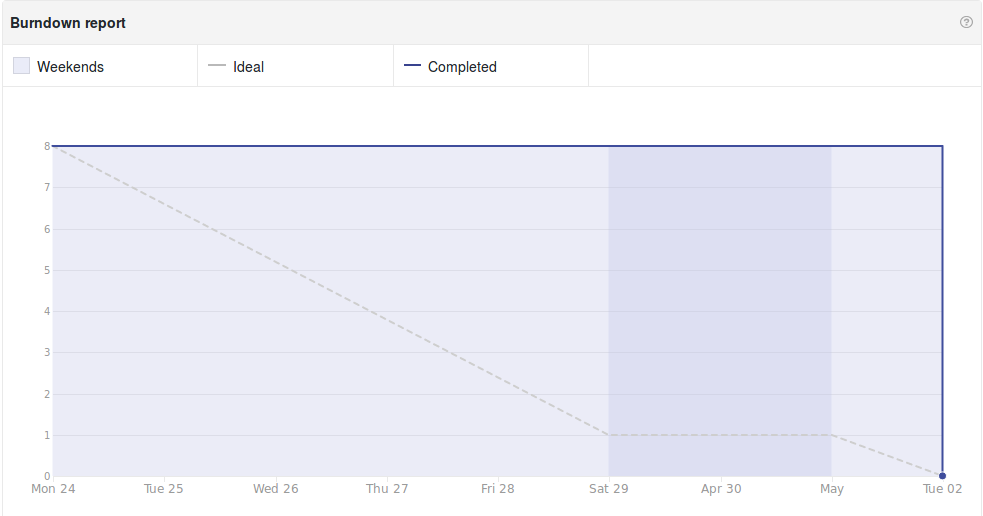
\includegraphics[width=\textwidth,height=7cm,keepaspectratio=true]{a_burndown_0}
    \caption[Gráfico burndown de la iteración 0]{Gráfico burndown de la iteración 0.}
    \label{fig:burndown0}
\end{figure}

En este caso el gráfico burndown de la figura \ref{fig:burndown0} muestra que todo el tiempo se fue con los problemas de la instalación de \textit{Unity} y que una vez completada el resto se terminó directamente.

\newpage
\subsection{Iteración 1: de 2-05-2017 hasta 7-05-2017}
En esta semana se empezó a trabajar con \textit{Unity}, se investigaron los ejemplos de prueba para crear el modelo del vehículo, se creó el primer algoritmo de planificación, el A*, y se investigó cómo se podían representar las rutas obtenidas en Unity llevándose a cabo su implementación.

Las tareas fueron:
\begin{itemize}
\item Crear el primer modelo de vehículo con movimiento y físicas de ruedas.
\item Crear el A*
\item Buscar cómo y realizar el dibujo de trayectorias.
\end{itemize}

\begin{figure}[htpb]
    \centering
    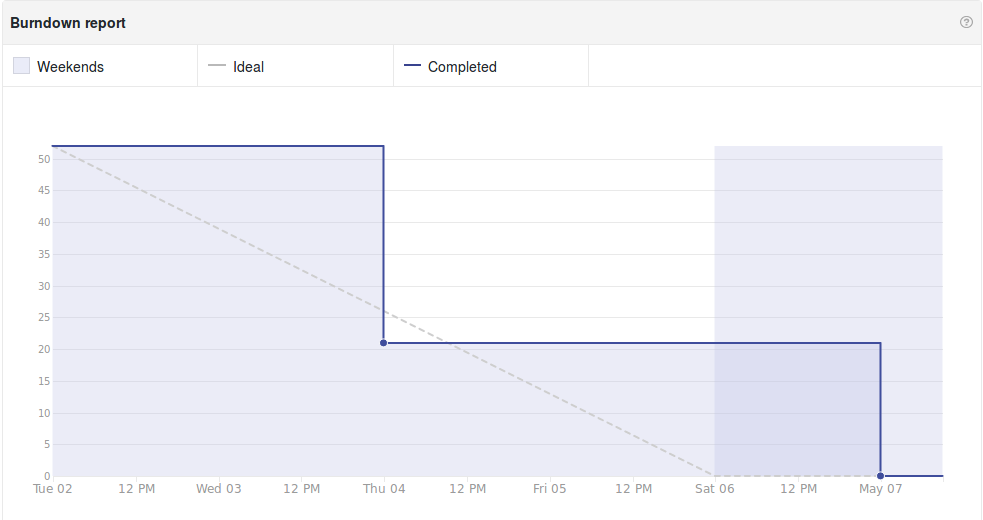
\includegraphics[width=\textwidth,height=7cm,keepaspectratio=true]{a_burndown_1}
    \caption[Gráfico burndown de la iteración 1]{Gráfico burndown de la iteración 1.}
    \label{fig:burndown1}
\end{figure}

El gráfico burndown de la figura \ref{fig:burndown1} muestra como se repartió el tiempo entre las dos tareas principales de estudiar los ejemplos de \textit{Unity} y realizar la implementación del A*.

\newpage
\subsection{Iteración 2: de 8-05-2017 hasta 15-05-2017}
Para esta semana se planificó terminar al A* y la representación de la trayectoria que se inició en la iteración anterior. Además, se investigó y se implementó la representación de los estados del A* para su visualización según se iba ejecutando el algoritmo. Por último, se planificó obtener el mapa de la escena de forma dinámica en tiempo de ejecución, que no fue posible debido a las limitaciones de la versión de \textit{Unity} utilizada, aunque se usó este trabajo y los conocimientos adquiridos sobre los \textit{Nav Mesh} para usarlos en el proyecto.

Las tareas fueron:
\begin{itemize}
\item Terminar A*.
\item Terminar la representación de la línea de trayectoria.
\item Crear la representación gráfica de la cuadrícula de los nodos de estado del A*.
\item Crear el mapa para el A* de forma dinámica según la escena.
\end{itemize}

\begin{figure}[htpb]
    \centering
    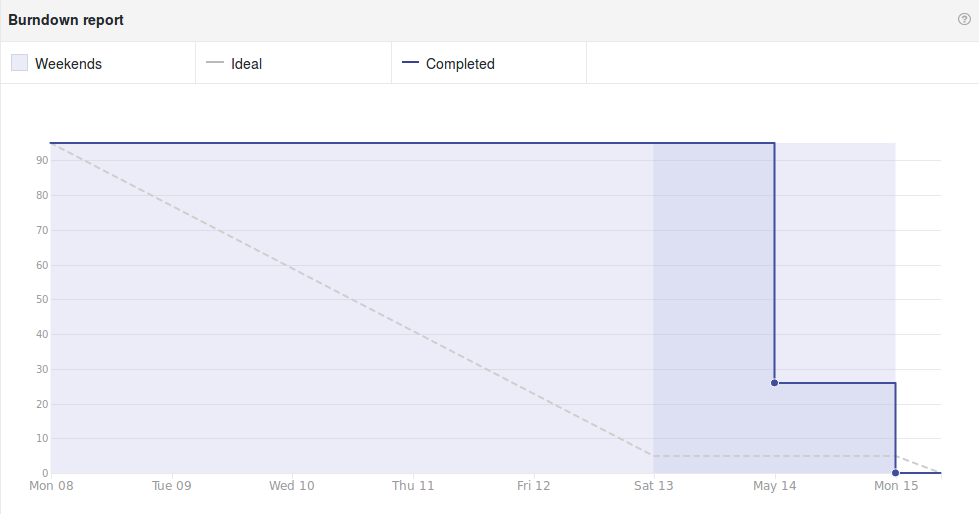
\includegraphics[width=\textwidth,height=7cm,keepaspectratio=true]{a_burndown_2}
    \caption[Gráfico burndown de la iteración 2]{Gráfico burndown de la iteración 2.}
    \label{fig:burndown2}
\end{figure}

El gráfico burndown de la figura \ref{fig:burndown2} muestra como la mayor parte del tiempo de esta iteración se utilizó en investigar el \textit{Nav Mesh} y la posible creación de los mapas de forma dinámica.

\newpage
\subsection{Iteración 3: de 16-05-2017 hasta 22-05-2017}
En esta iteración se implementó el \textit{Path Smoothing} para el suavizado de las rutas obtenidas. Se optimizó el rendimiento del A* a través del cambio de las estructuras de datos utilizadas, en concreto se buscó una implementación de una cola de prioridad. Se avanzó buscando documentación sobre \textit{PID Controller} para la próxima iteración, y se fue realizando la memoria con las secciones desarrolladas hasta ese momento.

Las tareas fueron:
\begin{itemize}
\item Implementar el \textit{Path Smoothing} al A*.
\item Optimizar el A*.
\item Buscar y leer documentación sobre el PID control.
\item Avanzar en la memoria.
\end{itemize}

\begin{figure}[htpb]
    \centering
    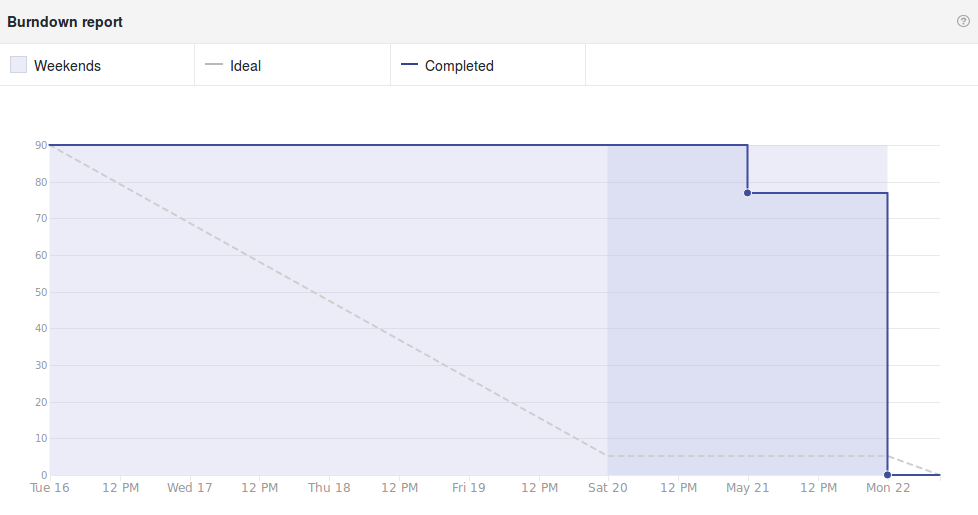
\includegraphics[width=\textwidth,height=7cm,keepaspectratio=true]{a_burndown_3}
    \caption[Gráfico burndown de la iteración 3]{Gráfico burndown de la iteración 3.}
    \label{fig:burndown3}
\end{figure}

En el gráfico burndown de la figura \ref{fig:burndown3} podemos observar que gran parte del tiempo de esta iteración se usó en la optimización del A* y en probar diferentes estructuras de datos, y la otra gran parte del tiempo se dedicó a realizar el \textit{Path Smoothing}.

\newpage
\subsection{Iteración 4: de 23-05-2017 hasta 30-05-2017}
Para esta iteración se utilizó la documentación de la semana anterior para desarrollar el \textit{PID Controller}. Para este semana se planificó realizar un \textit{PID Controller} para el control de las ruedas del vehículo.

También se implementaron dos nuevos algoritmos de búsqueda de rutas, el Theta* y el A* usando los vértices, que mejoraban al A* en la forma de las rutas obtenidas y en el rendimiento en el caso del A* de los vértices.

Se siguió realizando las secciones de la memoria correspondientes al trabajo realizado hasta el momento y se inició la creación de casos de test.

Las tareas fueron:
\begin{itemize}
\item Implementar \textit{PID Controller} para las ruedas y el motor.
\item Implementar algoritmo Theta*.
\item Implementar algoritmo A* con los vértices.
\item Avanzar con la memoria.
\item Empezar a crear casos de test.
\end{itemize}

\begin{figure}[htpb]
    \centering
    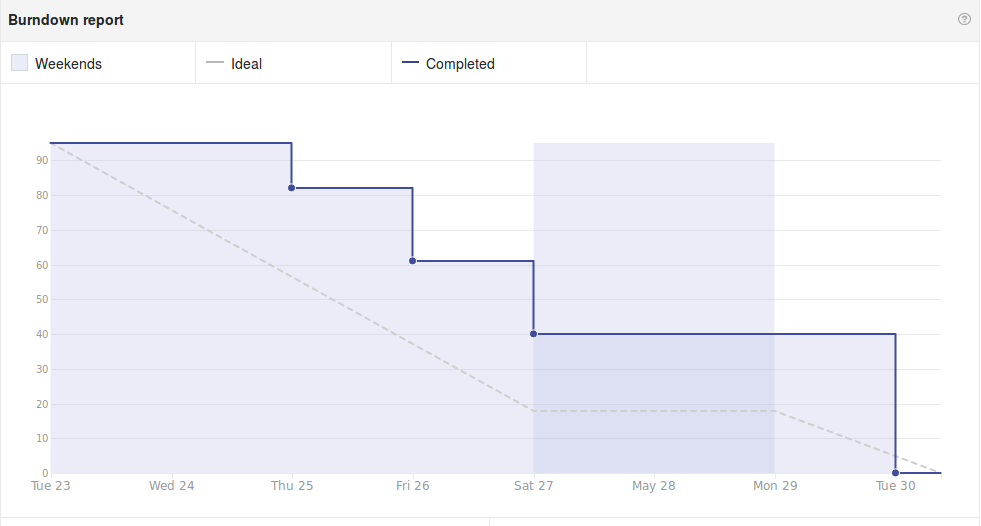
\includegraphics[width=\textwidth,height=7cm,keepaspectratio=true]{a_burndown_4}
    \caption[Gráfico burndown de la iteración 4]{Gráfico burndown de la iteración 4.}
    \label{fig:burndown4}
\end{figure}

En el gráfico burndown de la figura \ref{fig:burndown4} podemos ver como la semana se dividió principalmente entre la implementación de los algoritmos basados en al A* y la implementación del PID \textit{Controller}.

\newpage
\subsection{Iteración 5: de 31-05-2017 hasta 6-06-2017}
Para esta semana estaba planificado realizar un \textit{PID Controller} para el motor del vehículo, pero finalmente se decidió usar solamente el de las ruedas debido a que abarcaba los objetivos del proyecto por si mismo, moviendo el vehículo siguiendo la rutas obtenida, y utilizar en tiempo en otras tareas.

Se dedicó esta iteración a terminar las secciones de la memoria que se habían empezado las semanas anteriores, y a documentarse sobre el algoritmo \textit{Hybrid A*} para poder implementarlo en las siguientes iteraciones.

Las tareas fueron:
\begin{itemize}
\item Documentarse sobre la algoritmo Hybrid A* para implementarlo.
\item Avanzar en la memoria.
\end{itemize}

\begin{figure}[htpb]
    \centering
    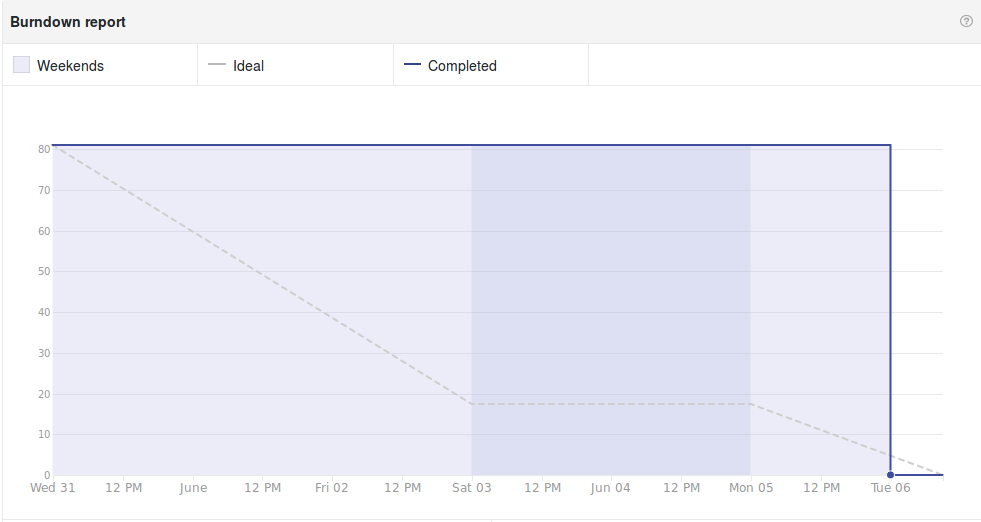
\includegraphics[width=\textwidth,height=7cm,keepaspectratio=true]{a_burndown_5}
    \caption[Gráfico burndown de la iteración 5]{Gráfico burndown de la iteración 5.}
    \label{fig:burndown5}
\end{figure}

En el gráfico burndown de la \ref{fig:burndown5} se muestra que el tiempo de esta semana se dedico a buscar documentación sobre el \textit{Hybrid A*}.

\newpage
\subsection{Iteración 6: de 7-06-2017 hasta 14-06-2017}
En esta iteración se implemento una primera versión del \textit{Hybrid A*}. Resulto complicado porque aún habiendo realizado buena parte de la documentación durante la semana anterior, no es un algoritmo que esté tan bien documentado y explicado como los anteriores. Finalmente se desarrollo una primera versión donde se calculaba la posición continua del vehículo y tenia en cuenta su rotación, pero resultaban rutas poco realistas y su movimiento a través del \textit{PID Controller} era limitado (por ejemplo, solo era capaz de ir adelante o hacia atrás no, cambiar de sentido).

También se utilizó parte del tiempo para realizar las correcciones a la memoria con los errores encontrados y las indicaciones de los tutores.

Las tareas fueron:
\begin{itemize}
\item Implementar el Algoritmo del \textit{Hybrid A*}.
\item Realizar las correcciones de la memoria.
\end{itemize}

\begin{figure}[htpb]
    \centering
    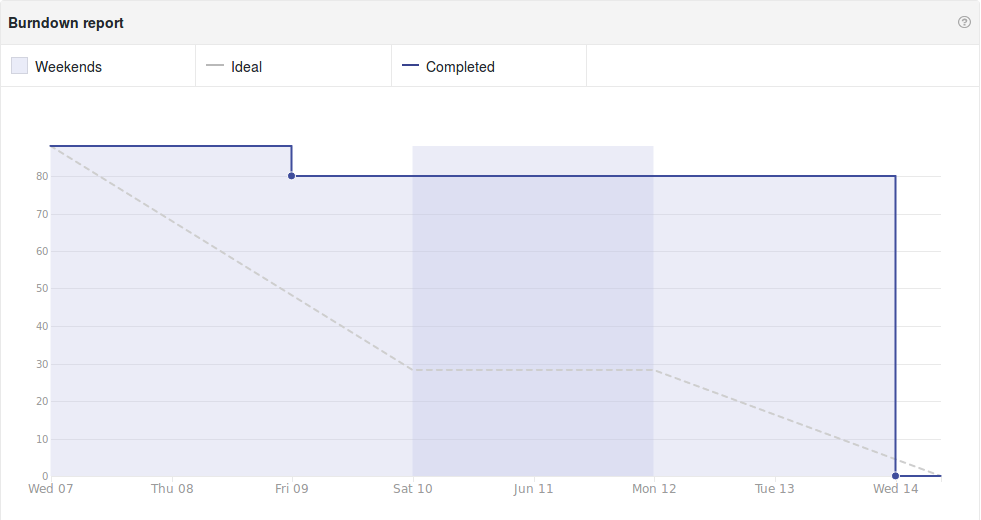
\includegraphics[width=\textwidth,height=7cm,keepaspectratio=true]{a_burndown_6}
    \caption[Gráfico burndown de la iteración 6]{Gráfico burndown de la iteración 6.}
    \label{fig:burndown6}
\end{figure}

En el gráfico burndown de la figura \ref{fig:burndown6} se muestra que tuvimos problemas en planificar las subtareas requeridas para le implementación del \textit{Hybrid A*} ya que aunque les estudiamos en la semana anterior fue complicado al ser un algoritmo del que no conocíamos nada de antemano y la dificultad de encontrar documentación detallada sobre le mismo.

\newpage
\subsection{Iteración 7: de 15-06-2017 hasta 19-06-2017}
Esta semana se dedicó a mejorar el \textit{Hybrid A*} para que el vehículo pudiera realizar maniobras. Para ello se modificaron las funciones del coste, se arreglaron los errores encontrados en la primera versión y se realizó un mapa de distancias. También fue necesario modificar el \textit{PID Controller} para que fuese capaz de seguir las rutas del \textit{Hybrid A*}. De esta manera se consiguió rutas más realistas que pudiera seguir el vehículo y que fuera capaz de realizar maniobras.

Además se siguió realizando la memoria con las secciones correspondientes al trabajo que se había ido realizando hasta el momento.

Las tareas fueron:
\begin{itemize}
\item Terminar el algoritmo del \textit{Hybrid A*}.
\item Avanzar en la memoria.
\end{itemize}

\begin{figure}[htpb]
    \centering
    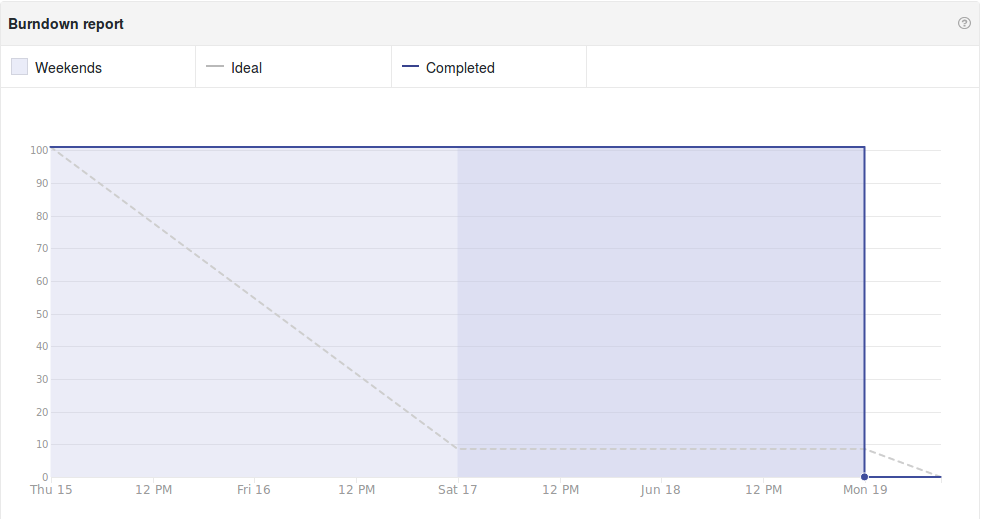
\includegraphics[width=\textwidth,height=7cm,keepaspectratio=true]{a_burndown_7}
    \caption[Gráfico burndown de la iteración 7]{Gráfico burndown de la iteración 7.}
    \label{fig:burndown7}
\end{figure}

Parecido a la semana anterior, el gráfico burndown de la figura \ref{fig:burndown7} muestra que una vez terminada la primera versión del \textit{Hybrid A*} que no funcionaba como deseábamos, se tuvo que investigar como poder arreglarlo sin tener las subtareas claras al inicio de la planificación.

\newpage
\subsection{Iteración 8: de 20-06-2017 hasta 26-06-2017}
Para esta semana principalmente se planificó terminar la memoria, añadiendo las últimas secciones, las imágenes, las tablas y los pseudocódigos.

Se finalizó el desarrollo del \textit{Hybrid A*} y se mejoró su rendimiento a través de la implementación de una nueva heurística que tiene en cuenta los obstáculos hasta la meta. Se mejoró el cálculo del coste corrigiendo los errores encontrados.

Las tareas fueron:
\begin{itemize}
\item Terminar la memoria y realizar las correcciones necesarias.
\item Mejorar heurística del \textit{Hybrid A*}.
\item Corregir errores en el cálculo de las heurísticas y el coste.
\end{itemize}

\begin{figure}[htpb]
    \centering
    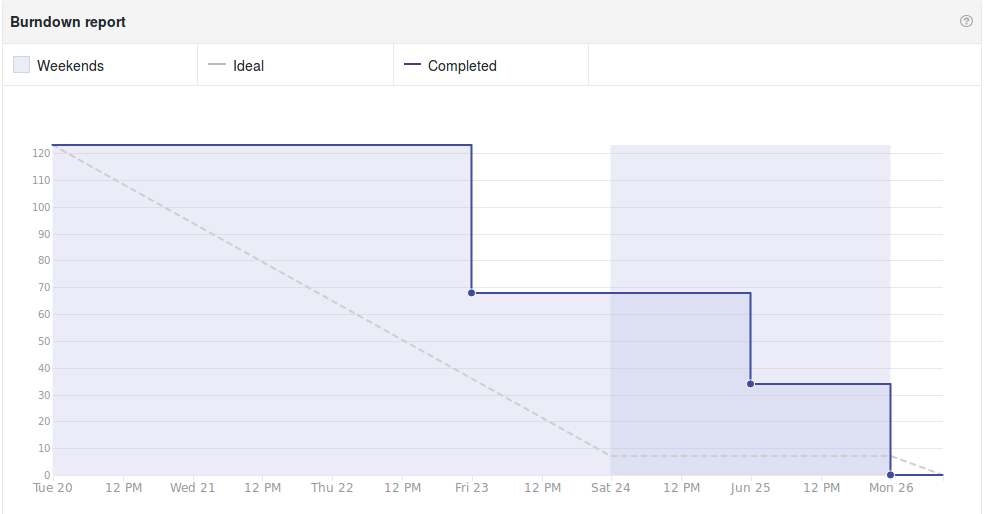
\includegraphics[width=\textwidth,height=7cm,keepaspectratio=true]{a_burndown_8}
    \caption[Gráfico burndown de la iteración 8]{Gráfico burndown de la iteración 8.}
    \label{fig:burndown8}
\end{figure}

El gráfico burndown de la figura \ref{fig:burndown8} muestra que en esta semana se planificó mejor las subtareas y el tiempo requerido por las mismas. La mayor parte del tiempo se dedicó a terminar la memoria y el resto a mejorar el \textit{Hybrid A*}.

\newpage
\subsection{Iteración 9: de 27-06-2017 hasta 3-07-2017}
En esta semana se termina el desarrollo del proyecto terminando las tareas pendientes.

Se realizaron los anexos y todas las secciones necesarias, se realizaron los vídeos con los resultados de distintas escenas, los casos de test, y la interfaz de usuario.

Las tareas fueron:
\begin{itemize}
\item Terminar los anexos.
\item Terminar los tests.
\item Implementar la GUI.
\item Realizar videos demostrativos.
\item Crear el póster de presentación.
\end{itemize}

El gráfico burndown de la figura A.10


\section{Estudio de viabilidad}

\subsection{Viabilidad económica}
En esta sección vamos a analizar el coste económico del proyecto y las posibles vías que pudiera tener para generar ingresos.

\subsubsection{Costes de personal}
El proyecto se ha llevado a cabo por una persona a tiempo completo durante dos meses. Hemos considerado que el salario neto rondaría los mil euros mensuales, y para calcular el coste total hemos considerado el porcentaje del salario de la Seguridad Social\footnote{Seguridad Social: \url{http://www.seg-social.es/Internet_1/Trabajadores/CotizacionRecaudaci10777/Basesytiposdecotiza36537/index.htm}} cuyo porcentaje es $31.2\%$ (contingencias comunes, contrato tiempo parcial y fondo de garantía social) , y del IRPF \footnote{IRPF: \url{http://www.agenciatributaria.es/static_files/AEAT/Contenidos_Comunes/La_Agencia_Tributaria/Informacion_institucional/Campanias/Retenciones_trabajo_personal/2017/Cuadro_tipo_retencion_2017.pdf}} cuyo porcentaje es $15\%$ para la elaboración de obras científicas.

\tablaSmall{Tabla de costes de personal}{l c}{tablacostepersonal}
{ \multicolumn{1}{l}{Coste} & Importe (\euro) \\}{ 
Salario mensual neto & 995.3 \\
IRPF & 277.5 \\
Seguridad Social & 577.2 \\
Salario Bruto & 1850 \\ \hline
\textbf{Total (2 meses)} & 3700 \\
}

En total el gasto por coste de personal para el proyecto es de 3700\euro.

\subsubsection{Costes de \textit{hardware}}
Para la realización del proyecto se ha utilizado un PC de sobremesa comprado en el año 2009 por un valor de 1000\euro \space aproximadamente. Vamos a considerar los meses transcurridos desde su compra como el tiempo para su amortización, en total 102 meses.

El coste amortizado de cada mes, por tanto, es de 9.8\euro, que por dos meses en total el coste del \textit{hardware} ha sido de 19.6\euro.

\subsubsection{Costes de \textit{software}}
Todo el \textit{software} utilizado ha sido \textit{software} libre o gratuito, incluido el sistema operativo que ha sido Xubuntu 16.04, por lo que el coste del \textit{software} ha sido de 0\euro.

\subsubsection{Otros costes}
La realización del proyecto lleva consigo otros costes adicionales que son necesarios para su realización. Hemos considerado el alquiler de un lugar para su realización de un coste aproximado de 500\euro\space mensuales, el coste del proveedor de internet necesario en 50\euro\space mensuales, y el coste de imprimir las memorias, el póster y los DVDs en 60\euro\space.

\tablaSmall{Tabla de otros costes}{l c}{tablaotroscostes}
{ \multicolumn{1}{l}{Otros costes} & Importe (\euro) \\}{ 
Internet & 50 \\
Impresos y DVDs & 60 \\
Alquiler & 500 \\ \hline
\textbf{Total (2 meses)} & 1160 \\
}

En total, el coste de estos otros gastos suman un total de 1160\euro\space.

\subsubsection{Total costes del proyecto}
El total de todos los costes del proyecto asciende a un total de 4879.6\euro.

\tablaSmall{Costes totales}{l c}{tablacostestotales}
{ \multicolumn{1}{l}{Costes} & Importe (\euro) \\}{ 
Personal & 3700 \\
\textit{Hardware} & 19.6 \\
\textit{Software} & 0 \\
Otros & 1160 \\ \hline
\textbf{Total} & 4879.6 \\
}

\subsubsection{Ingresos}
En un principio no se ha desarrollado la aplicación para que genere beneficios de ningún tipo, la intención del desarrollo ha sido de investigación y aprendizaje. De todas formas, la forma posible del obtener ingresos y rentabilizar el proyecto sería a través de la venta en la \textit{Unity Store}\footnote{Unity Store: \url{https://store.unity3d.com/}} de la implementación de los algoritmos como un \textit{asset} para otros proyectos.

Teniendo en cuenta el coste de 4879.6\euro, con un precio de 30\euro, y que \textit{Unity} en las condiciones legales\footnote{Unity Store, condiciones legales: \url{https://unity3d.com/es/legal/as_provider}} para usar su \textit{Store} retiene un $30\%$, no recuperaríamos la inversión hasta alcanzar las 233 unidades vendidas.

\subsection{Viabilidad legal}
En esta sección vamos a analizar la viabilidad legal de las licencias usadas en el proyecto así como las licencias con las que se distribuirá.

El motor \textit{Unity}\cite{unityweb} podemos usarlo libremente en su versión Personal siempre que no superemos unos ingresos de 100 mil dolares al año. En cuanto a \textit{Unity} y sus \textit{assets}, se pueden usar libremente dentro del proyecto\footnote{Unity Store EULA: \url{https://unity3d.com/es/legal/as_terms}} según los términos legales de la \textit{Unity Store}.

La librería externa que hemos usado ha sido la de la cola de prioridad en C\# \textit{High Speed Priority Queue for C Sharp}\footnote{Cola de prioridad: \url{https://github.com/BlueRaja/High-Speed-Priority-Queue-for-C-Sharp}}\cite{bluerajacola} que tiene una licencia de uso MIT \footnote{Licencia cola de prioridad: \url{https://github.com/BlueRaja/High-Speed-Priority-Queue-for-C-Sharp/blob/master/LICENSE.txt}} que nos permite usarla libremente incluso con fines comerciales.

Con lo cual, la limitaciones que nos encontramos en materia legal serían en caso de comercializar el proyecto, el límite de 100 mil dolares de \textit{Unity}, y tener en cuenta que los \textit{assets} solo se nos permite usarlos como una parte del proyecto, no podemos modificarlos y distribuirlos o venderlos de forma separada.

En cuanto a las licencia del código del proyecto se ha elegido la licencia GPL 3.0, de tal forma que los usos posteriores del código respeten la misma licencia y que deban distribuir el código fuente. Ya que no se ha desarrollado con una intención comercial, si no con intención de investigación y aprendizaje, y debido al uso que hemos dado al código abierto de otras fuentes (programas, ejemplos y la cola de prioridad) para desarrollarlo, consideramos que es la opción más adecuada.

En cuanto a la memoria y la documentación, hemos elegido por los mismo motivos una licencia \textit{Creative Commons} CC BY-NC\footnote{Licencias Creative Commons\url{https://creativecommons.org/licenses/?lang=es_ES}} que permite su uso en cualquier modo siempre que se reconozca la autoría y no se use en obras comerciales.
\apendice{Especificación de Requisitos}

\section{Introducción}

\section{Objetivos generales}

\section{Catalogo de requisitos}

\section{Especificación de requisitos}



\apendice{Especificación de diseño}

\section{Introducción}
En esta sección se va a explicar como se ha diseñado la aplicación para que realice los objetivos y requisitos de la misma. También se mostrarán los diagramas correspondientes, aunque se han simplificado omitiendo algunos elementos como los atributos o métodos para mejorar su representación.

\section{Diseño de datos}
La aplicación se divide en dos grandes bloques. Por una parte están los algoritmos que planifican la ruta y por otra están las clases que se dedican a realizar tareas con las rutas que devuelven los algoritmos.

La clase MoverCoche es la clase principal y se encarga de seleccionar el algoritmo, recoger la ruta y proporcionarsela en orden a las clases de suavizado, PathSmoothing, y de movimiento, PIDControl.

También se encarga de instanciar e iniciar las clases auxiliares y parámetros necesarios, y es desde MoverCoche donde se sigue el bucle continuo del motor gráfico para realizar las operaciones.

\begin{figure}[htpb]
    \centering
    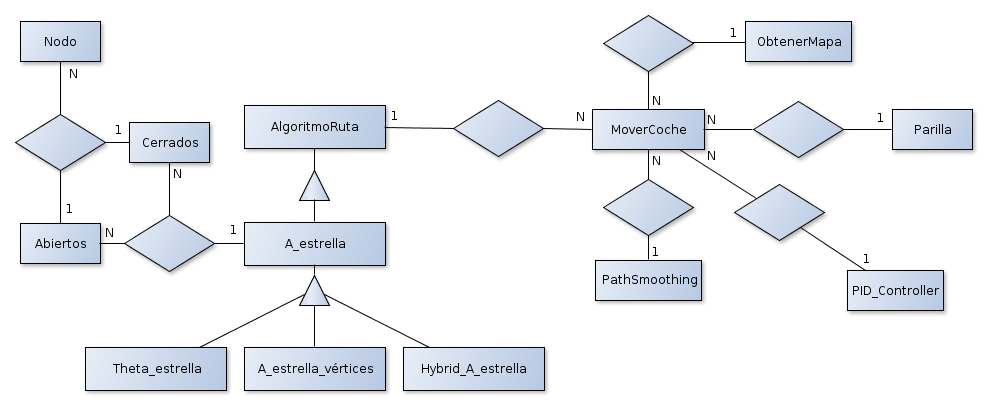
\includegraphics[width=\textwidth,height=10cm,keepaspectratio=true]{c_entidad_relacion}
    \caption[Diagrama entidad relación]{Diagrama entidad relación.}
    \label{fig:centidadrelacion}
\end{figure}

\section{Diseño procedimental}
\textit{Unity} como motor gráfico forma parte de la aplicación. La forma de usar \textit{Unity} es a través de \textit{scripts} que heredan de la clase \textit{MonoBehaviour} y enlazandoles con algún elemento de la escena que hayamos creado.

Las clases que heredan de \textit{MonoBehaviour} tienen varios métodos que permiten ser usados cuando se inicia la ejecución, y desde ese punto llamar al resto de clases y métodos. Para este proyecto hemos usado los métodos \textit{Start()}, \textit{FixedUpdate()} y \textit{Update()}.
\begin{itemize}
\item \textbf{\textit{Start()}}: este método se ejecuta cuando se cargue en la escena el objeto al que esta enlazado. Se utiliza para la inicialización de elementos.
\item \textbf{\textit{FixedUpdate()}}: este método se ejecuta a intervalos de tiempo cortos (más rápido que un \textit{frame}), y se utiliza para el cálculo de las físicas.
\item \textbf{\textit{Update()}}: este método se ejecuta cada \textit{frame}, y se utiliza para toda la lógica que no involucre a las físicas.
\end{itemize}

El vehículo se carga al inicio de la ejecución puesto que está presente en la escena que hemos creado, y por tanto, el primer método que se ejecutará será el \textit{Start()} del \textit{script} MoverCoche que tiene enlazado. Se usa para iniciar todo lo necesario para realizar tanto la ejecución de los algoritmos de búsqueda de rutas, como las clases que hacen uso de la ruta como \textit{PathSmoothing} y \textit{PIDControl}. Es aquí también donde dependiendo de las opciones seleccionados se elegirá un algoritmo u otro para el cálculo de la ruta.

A continuación, el programa se ejecuta como un bucle continuo donde se están constantemente llamando a \textit{Update()} y \textit{FixedUpdate()}. Se ha usado \textit{Update()} para realizar la búsqueda de la ruta, de tal forma que cada llamada a \textit{Update()} corresponde con un ciclo del algoritmo correspondiente. En cada una de esas llamadas también se dibujan el progreso del algoritmo en su búsqueda. \textit{FixedUpdate()} no se utiliza hasta que se ha obtenido una ruta. Al ser usado para el cálculo de las físicas, y por tanto de la simulación del vehículo y su movimiento, hasta que no haya una ruta que seguir no se hace uso de él. Cuando ya se ha obtenido una ruta, se deja de usar \textit{Update()}, y se pasa a mover el vehículo desde \textit{FixedUpdate()}.

\begin{figure}[htpb]
    \centering
    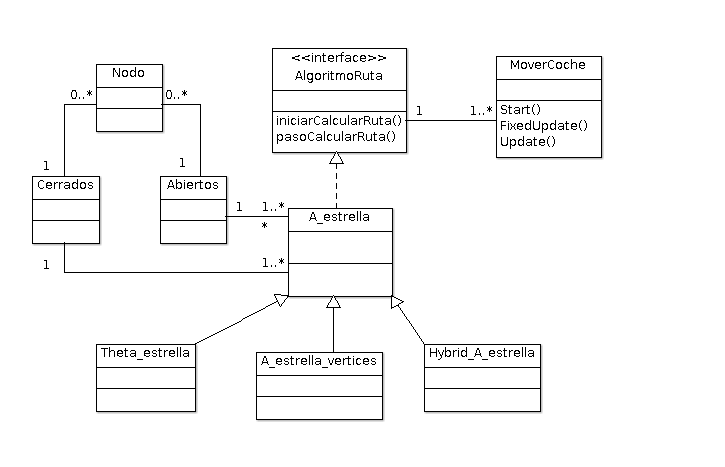
\includegraphics[width=\textwidth,height=10cm,keepaspectratio=true]{c_clases_algoritmos}
    \caption[Diagrama de clases de los algoritmos]{Diagrama de clases de los algoritmos.}
    \label{fig:cclasesalgoritmos}
\end{figure}

Se ha creado la interfaz AlgoritmoRuta para que en el futuro, implementando los métodos de la interfaz, se pueda instanciar el algoritmo elegido en MoverCoche con lo que facilite la creación de algoritmos nuevos. En el caso de los algoritmos que se han implementado, son tanto el A* como algoritmos que modifican el A*, por lo que hemos usado el A* y se han ido modificando en las subclases los métodos que fueran necesarios.

\begin{figure}[htpb]
    \centering
    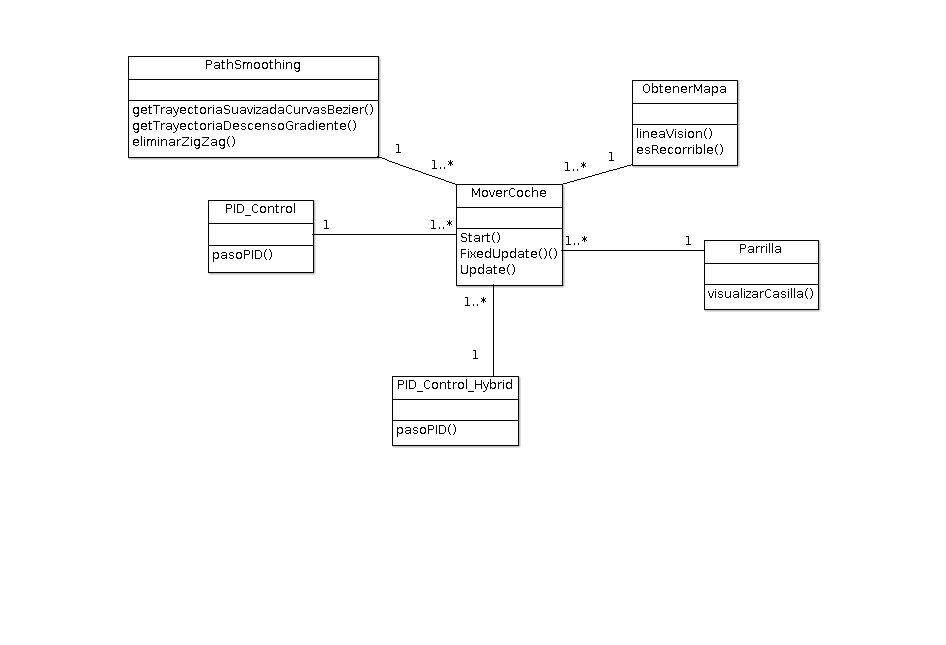
\includegraphics[width=\textwidth,height=10cm,keepaspectratio=true]{c_clases_rutas}
    \caption[Diagrama de clases del manejo de las rutas]{Diagrama de clases del manejo de las rutas.}
    \label{fig:cclasesrutas}
\end{figure}

Una vez obtenida la ruta, se pasa a la siguiente fase de la ejecución. En primer lugar se suaviza la ruta con los métodos de \textit{PathSmoothing}, y a continuación se realiza el movimiento del vehículo. Para el movimiento se realiza desde \textit{FixedUpdate()}, como comentamos anteriormente, y de igual manera se realiza paso a paso en cada una de sus ejecuciones. Para el movimiento autónomo, se llama en cada ejecución a \textit{PIDControl} pata que actualice los valores necesarios para el motor y las ruedas teniendo en cuenta el desplazamiento que ha ocurrido desde la anterior iteración.

\section{Diseño arquitectónico}
En la figura \ref{fig:cdiagramasecuencia} podemos observar como se relacionan todas las clases principales a partir de MoverCoche.

Las dos primeras llamadas, \textit{iniciarCalcularRuta()} y \textit{getMapaDistancias()}, se ejecutan en el método \textit{Start()} fuera del bucle continuo del motor gráfico. Con \textit{iniciarCalcularRuta()} se prepara para iniciarse el algoritmo, creando todos los elementos que necesite. En este ejemplo obtenemos el mapa de distancias puesto que se crea al iniciarse el \textit{Hybrid A*} ya que lo necesita durante su ejecución.

A continuación, se  realiza la llamada a \textit{pasoCalcularRuta()}, que se ejecuta en \textit{Update()}, formando ya parte del bucle continuo. Al ser \textit{Update()}, se ejecutan una vez por cada frame. Es aquí donde se realiza la búsqueda de la ruta por parte del algoritmo y dibuja el progreso de su ejecución. Cuando termina la búsqueda, en ese ciclo se llama a \textit{getTrayectoriaDescensoGradiente()} para suavizar el resultado.

Y por último, la llamada a \textit{pasoPID()} se realiza en \textit{FixedUpdate()}, que se ejecuta a un intervalo fijo de tiempo, más rápido que a cada \textit{frame}. Como es el método destinado al cálculo de las físicas, se realiza la llamada a \textit{pasoPID()} para obtener los valores de la fuerza del motor y del giro de las ruedas para que el vehículo se mueva de una forma autónoma.

\begin{figure}[htpb]
    \centering
    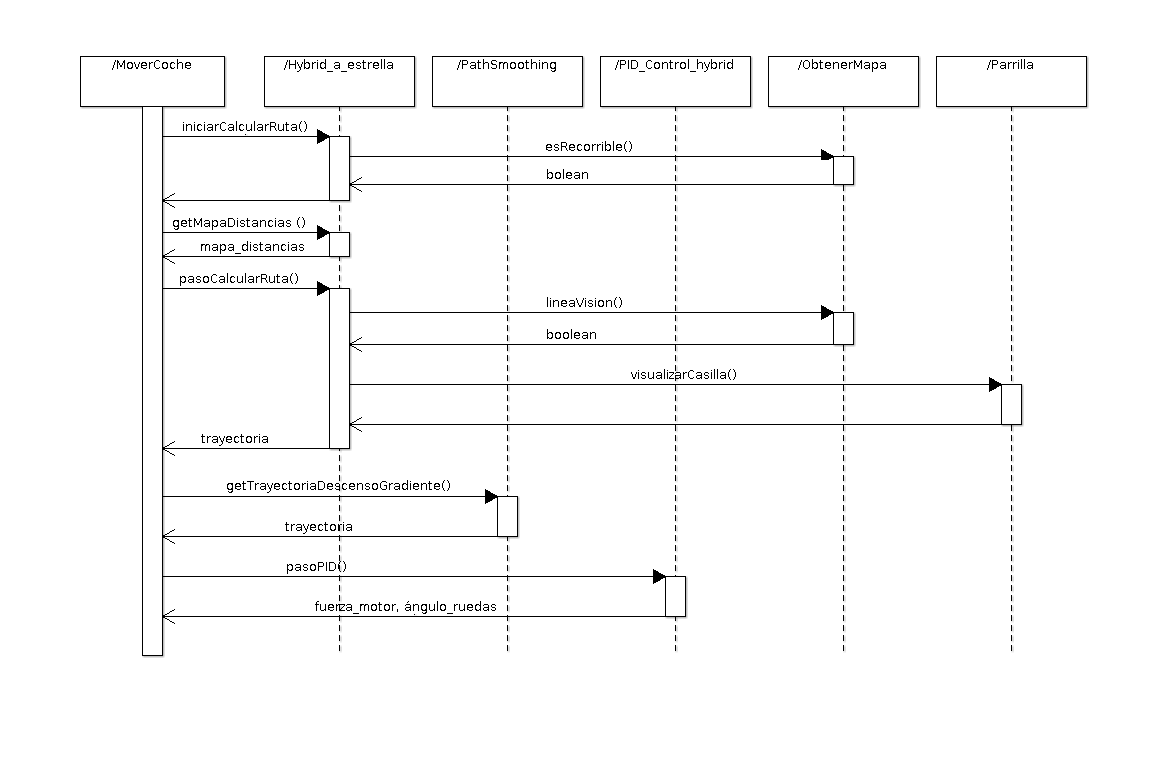
\includegraphics[width=\textwidth,height=20cm,keepaspectratio=true]{c_diagrama_secuencia}
    \caption[Diagrama de secuencia]{Diagrama de secuencia usando el algoritmo \textit{Hybrid A*}.}
    \label{fig:cdiagramasecuencia}
\end{figure}



\apendice{Documentación técnica de programación}

\section{Introducción}

\section{Estructura de directorios}

\section{Manual del programador}
Instalación Unity:

Unity en su versión linux puede instalarse de dos maneras: con el archivo .deb y a través de un instalador en forma de script. Ambos archivos se suministran desde la web oficial y se pueden obtener desde el siguiente enlace:

\href{https://forum.unity3d.com/threads/unity-on-linux-release-notes-and-known-issues.350256/}{Web oficial con las versiones de Unity para linux}

La versión utilizada ha sido la 5.3.6f1 que se puede encontrar en:

\href{https://forum.unity3d.com/threads/unity-on-linux-release-notes-and-known-issues.350256/#post-2717623}{Post de la web oficial para la versión 5.3.6f1}

Y descargar de los siguientes enlaces:

Archivo deb: \href{http://download.unity3d.com/download_unity/linux/unity-editor-5.3.6f1+20160720_amd64.deb}{Archivo deb para versión 5.3.6f1}

Instalador: \href{http://download.unity3d.com/download_unity/linux/unity-editor-installer-5.3.6f1+20160720.sh}{Instalador para versión 5.3.6f1}

Ambos archivos: \href{http://files.unity3d.com/levi/unity-editor-5.3.6f1+20160720.torrent}{Archivo torrent con ambos archivos}

Para realizar la instalación hemos usado el archivo instalador con los siguientes pasos:
1 Darle permisos de ejecución con chmod +x al archivo instalador
2 Ejecutar el archivo como superusuario. Crea un diretorio donde lo ejecutemos donde se encontraran todos los archivos de Unity.

Para ejecutarlo hay que ir al nuevo directorio que creo el instalador y ejecutar el ejecutable del editor de Unity que se encuentra dentro de Editor/ 

Para poder usar Monodevelop con la version de Unity, hay que instalar ademas de la versión que viene con el instalador el resto de archivos de monodevelop. Con el comando sudo apt-get install mono-complete se instalan desde los repositorios todos los archivos necesarios.

Para comprobar que Unity abrirá el monodevelop con su versión para unity desde el menu Edit->Preferences, en la seccion External Tools, comprobamos que el editor de  los scripts seleccionado es internal. Aunque se puede usar cualquier editor para realizar los scripts, es recomendable usar monodevelop de este forma porque hay diferencias entre los lenguajes de programación estandar y las versiones de ellos que usa Unity.

Instalación SmartGit:

Para al organización el repositorio hemos elegido SmartGit, que es un programa disponible de forma gratuita para uso no comercial con versión para linux.

Para su instalación hay que descargarse el archivo deb de su página web

\href{https://www.syntevo.com/smartgit/download}{Página de SmartGit}

La versión que hemos utilizado es la 17.0.3 que se puede descargar del siguiente enlace:

\href{https://www.syntevo.com/smartgit/download?file=smartgit/smartgit-17_0_3.deb}{Archivo deb de SmartGit 17.0.3}

El modo de instalación que hemos usado es haciendo doble click sobre el archivo deb abriendolo con el Instalador de software de ubuntu. También se puede instalar con el comando dpkg -i nombre-archivo.deb.

Instalación de texmaker:
Texmaker lo hemos instalado desde los repositorios de ubuntu usando el gestor con interfaz gráfica synaptic.

También se puede instalar con el comando apt-get install textmaker.

Instalación ZenHub:

Para la planificación y control del proyecto hemos usado Zenhub sobre github. Es un addons de firefox que añade funciones como las boards para manejar el control de las issues y las milestones del proyecto, y que permite ver los gráficos del progreso que se ha realizado.

Para instalarlo, hay que ir a la web oficial
/href{https://www.zenhub.com/}{Web oficial ZenHub}

Pulsando sobre el botón de añadir ZenHub a Github, Firefox nos preguntará si queremos permitir a esa web instalar complementos y debemos darle permiso. A continuaciñon se instalará en firefox de forma automática y cuando vayamos a nuestro proyecto en github tendremos disponibles la funciones adicionales.

\section{Compilación, instalación y ejecución del proyecto}

\section{Pruebas del sistema}

\apendice{Documentación de usuario}

\section{Introducción}
En esta sección se va detallar como utilizar la aplicación. Como usuarios hay dos posibilidades. La versión ejecutable, que permite ver una serie de escenarios de prueba, y usar la aplicación directamente desde \textit{Unity}, lo que permite poder modificar las escenas, los parámetros y contar con una vista adicional para poder seguir el desarrollo de los algoritmos.

\section{Requisitos de usuarios}
Para poder ejecutar el proyecto desde \textit{Unity}, es necesario la versión 5.3.6 o superior, y un ordenador con cualquiera de los sistemas operativos principales (Linux, Windows y MacOS) que cuente con una tarjeta gráfica 3D.

Para el ejecutable los requisitos son los mismos solo que no es necesario usar \textit{Unity}.

Los requisitos mínimos oficiales para usar \textit{Unity} son:\footnote{Requisitos mínimos Unity: \url{https://unity3d.com/es/unity/system-requirements}}
\begin{itemize}
\item Sistema operativo Windows 7 SP1 o superior, MacOS X 10.8 o superior, Ubuntu 12.04 o superior.
\item Tarjeta gráfica con DX9 (modelo de shader 3.0) o DX11 con capacidades de funciones de nivel 9.3.
\item CPU compatible con el conjunto de instrucciones SSE2.
\end{itemize}

\section{Instalación}
El proceso de instalación para usar la aplicación con el editor de \textit{Unity} es la misma que vimos en la sección \ref{dinstalacion}.

Todos los archivos necesarios están en el repositorio de github, cuya dirección es: \href{https://github.com/vpe0001/Algoritmos\_de\_busqueda\_3D-Unity}{Repositorio del proyecto}\footnote{Repositorio del proyecto: \url{https://github.com/vpe0001/Algoritmos\_de\_busqueda\_3D-Unity}}

Para descargarlo, se puede usar git o descargar el archivo zip y descomprimir los ficheros. Desde \textit{Unity}, se abre el proyecto que se encuentra en la carpeta \textit{Codigo\textbackslash Algoritmos\_de\_busqueda\_3D}, o bien se crea un proyecto nuevo y se importa el paquete del directorio \textit{Exportar}, desde \textit{Assets-\textgreater Import Package}.

El ejecutable no requiere de instalación adicional. Los archivos ejecutables se encuentran en la carpeta\textit{Build}, en la que a su vez hay dos carpetas, una para la versión Linux, y otra para la versión Windows.

\section{Manual del usuario}
\subsection{Manual para \textit{Unity}}
Una vez realizada la instalación, abriremos el proyecto con \textit{Unity}. Cuando se inicie, nos encontremos en la interfaz del editor de \textit{Unity}. Desde \textit{File-\textgreater Open Scene} podemos cargar la escena que deseemos probar. Nos encontraremos una pantalla similar a la de la figura \ref{fig:dunityui}.

\begin{figure}[htpb]
    \centering
    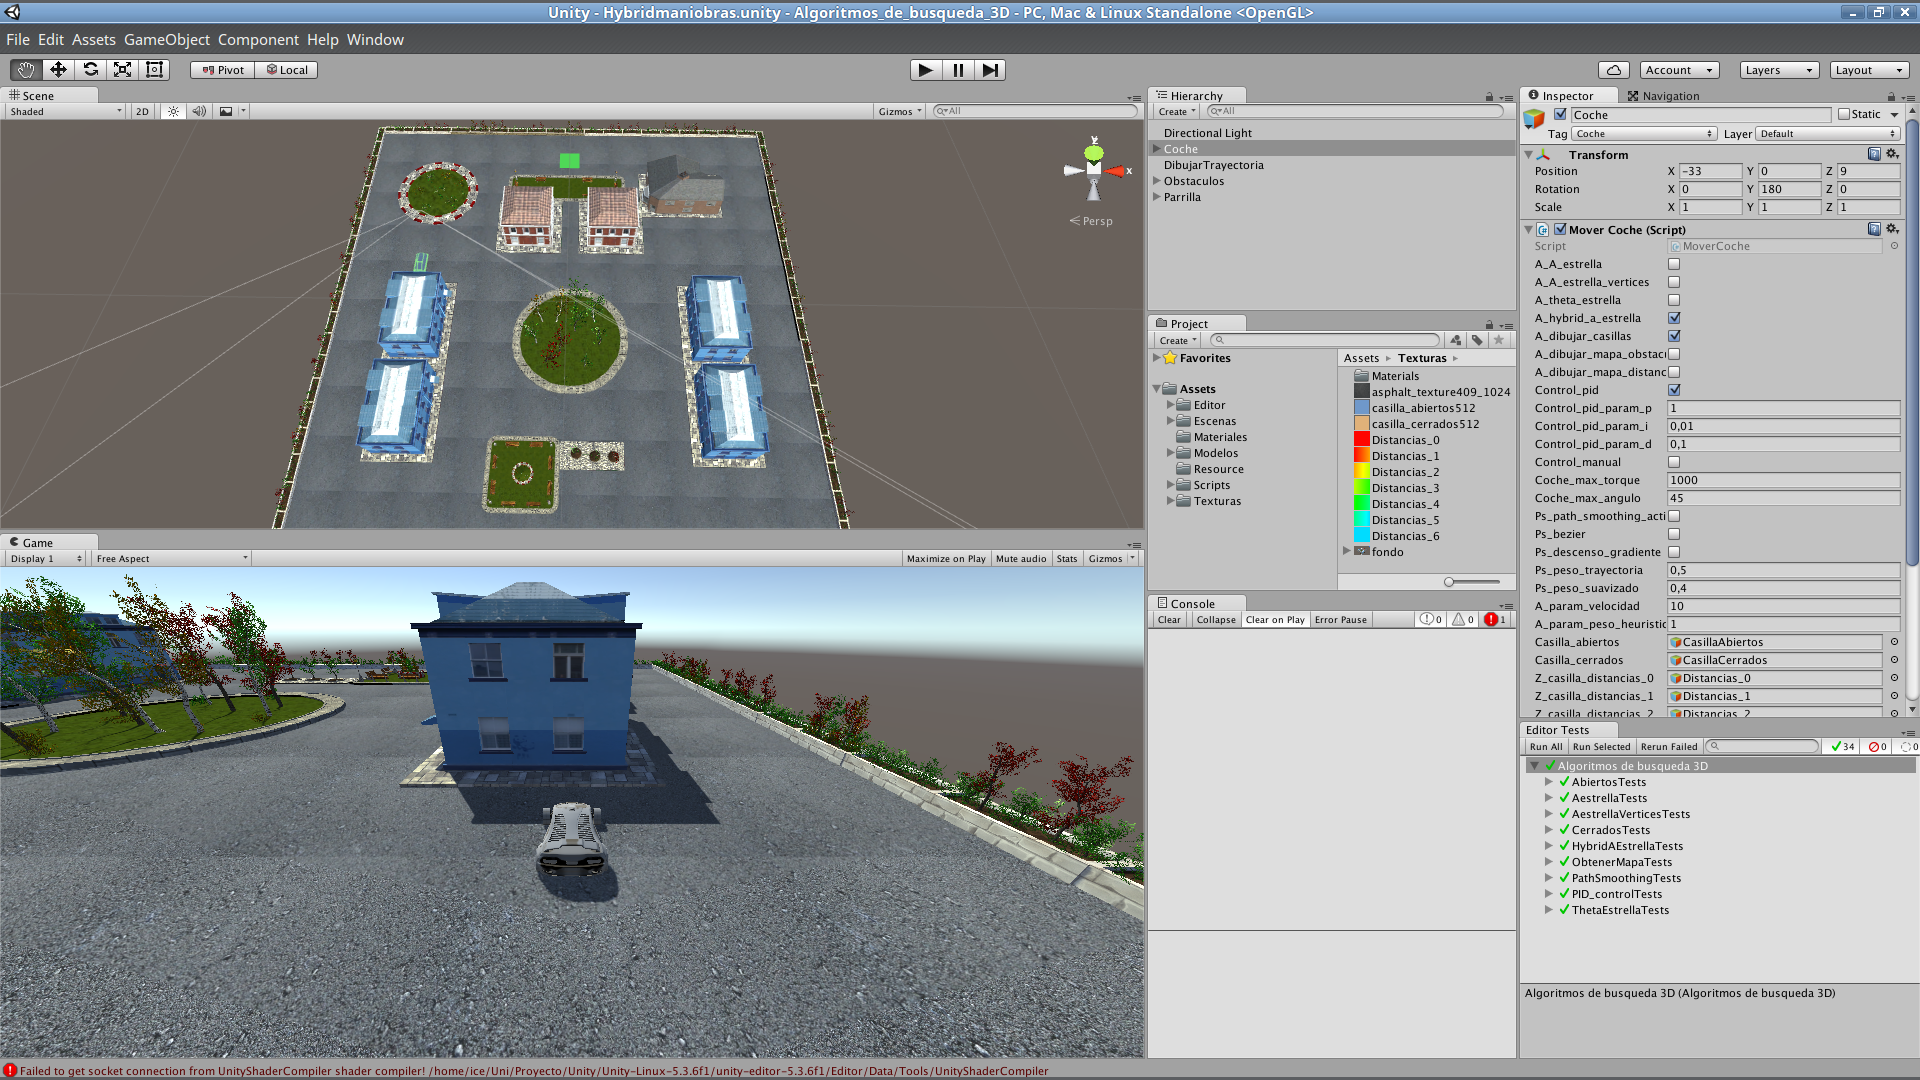
\includegraphics[width=\textwidth,height=8cm,keepaspectratio=true]{d_unityui}
    \caption[Pantalla de la interfaz de \textit{Unity}]{Pantalla de la interfaz de \textit{Unity}.}
    \label{fig:dunityui}
\end{figure}

A la izquierda, tenemos dos vistas de la escena en tres dimensiones. La de arriba corresponde al editor, y nos permite colocar la cámara en cualquier momento donde deseemos haciendo \textit{click} con el ratón. Esta vista es útil para tener un perspectiva de la escena completa, y poder observar como se desarrollan los algoritmos por ella. En la vista de abajo se encuentra la perspectiva desde el vehículo. Esta vista es útil cuando se realiza el seguimiento de la ruta, para poder observar el desplazamiento del vehículo.

Las dos columnas de la derecha corresponden a los elementos del proyecto. \textit{Hierarchy} contiene los elementos de la escena que podemos seleccionar para modificarles, mientras que \textit{Project} muestra todos los \textit{assets} del proyecto que podemos usar para crear las distintas escenas.

\textit{Inspector} mostrará los parámetros de los elementos seleccionados, y es donde vamos a modificar los distintos valores de los algoritmos. Seleccionando Coche en \textit{Hierarchy} y nos mostrará los valores que podemos configurar en el proyecto:
\begin{itemize}
\item \textbf{\textit{Transform}}: donde podemos modificar la posición (los valores de \textit{Position}) y la orientación del vehículo (el valor $y$ de \textit{Rotation}). También está disponible para el resto de los elementos como los obstáculos
\item A continuación aparecen los cuatro algoritmos disponibles para seleccionar: el A*, Theta*, A* con vértices y Hybrid A*.
\item Las opciones de \textit{dibujar mapa obstáculos} y \textit{dibujar mapa distancias} muestran respectivos mapas al inicio de la ejecución. Aunque no es recomendable realizar la ejecución completa con los mapas activados puesto que, además de perder visibilidad, el rendimiento debido al gran número de elementos en pantalla se reduce considerablemente.
\item La opción siguiente nos permite activar el \textit{PID Controller} para el movimiento autónomo del vehículo, y podemos modificar los parámetros \textit{P}, \textit{I} y \textit{D} para comprobar como afectan al movimiento.
\item Control manual nos permite, una vez activado, manejar al vehículo con las teclas del teclado.
\item Con \textit{Path Smoothing} activamos el suavizado de la ruta. Si no activamos las opciones de \textit{Descenso Gradiente} ni \textit{Curvas Bézier}, realizará la eliminación del zigzag. Si no, realizará la opción seleccionada. También es posible modificar los valores de los parámetros del \textit{Descenso gradiente} y ver las distintas rutas que genera.
\item La opción de \textit{param velocidad} se utiliza cuando no se ha seleccionado ni \textit{PID control} ni \textit{control manual}. En ese caso el vehículo no se moverá a usando las físicas, si no que se trasladará a través de la ruta hasta la meta a la velocidad que indica ese parámetro.
\item El parámetro \textit{peso heurísticas} sirve para configurar cuanta importancia tendrá la función H() en las rutas generadas en relación a la función G(). Si el valor es grande, el algoritmo búscará más en anchura, mientras que si es pequeño, intentará antes acercarse a la meta.
\end{itemize}

\subsection{Manual para el ejecutable}
La versión ejecutable es una aplicación reducida de lo que se puede hacer desde \textit{Unity}. Consiste en un menú principal donde se pueden escoger ocho escenas preconfiguradas.

Para ejecutarlo se hace doble \textit{click}, a continuación aparecen las opciones gráficas de resolución y preajustes de calidad de la imagen disponibles. Pulsando aceptar se inicia el menú de la aplicación, como se muestra en la figura \ref{fig:dmenuejecutable}\footnote{\textit{Unity} no permite el uso de acentos en los elementos de texto para la interfaz}.

\begin{figure}[htpb]
    \centering
    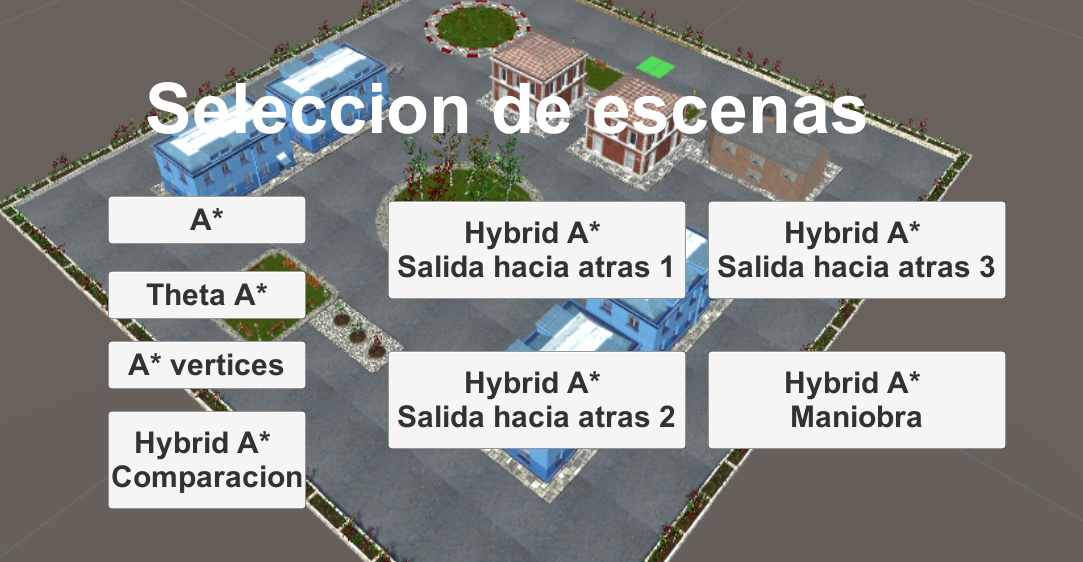
\includegraphics[width=\textwidth,height=8cm,keepaspectratio=true]{d_menuejecutable}
    \caption[Pantalla del menú del ejecutable]{Pantalla del menú del ejecutable.}
    \label{fig:dmenuejecutable}
\end{figure}

Para usarlo, hacemos \textit{click} en el botón correspondiente y se ejecutará la escena asociada. Cuando el vehículo llegue a la meta, la ejecución habrá terminado y se puede cerrar la ventana. Para cargar otra escena repetimos el proceso.

La columna de botones de la izquierda corresponden al mismo escenario, pero cada uno con un algoritmo diferente para poder compararles. Los cuatro botones restantes corresponden al \textit{Hybrid A*}, donde el vehículo realiza distintas maniobras.




\bibliographystyle{plain}
\bibliography{bibliografiaAnexos}

\end{document}
